\section{Semantic LSP}%
\label{sec:semantic_lsp}

When developing a LSP, we made sure to follow the state of the art best implementation practices\cite{10.1145/3550355.3552452,10.1145/3563834.3567537,10.1145/3550355.3552452,Bour_2018}.
Semantic LSP is built on top of an entity component system, allowing for even greater seperation of concern than the proposed \textit{Layered Architecture}\cite{10.1145/3550355.3552452}.

Entity component system is a software pattern that involves breaking your program up into Entities, Components, and Systems.
Entities are unique "things", here documents, that are assigned groups of Components, which are then processed using Systems.
Components include the contents of the source file, the location of the source file, the derived triples, etc.
Systems are functions that are grouped in schedules, one system might derive defined owl properties from derived triples and might be present in the \textit{Parse} schedule.
Each language can then add their specific systems into the defined schedules for language specific functionality.
This way common systems are defined once, resulting in a consistent experience over all semantic languages.
Bour et al. state "No spec, no tests"\cite{Bour_2018}, meaning it is difficult to write a useful testsuite for language servers.
User-facing features are not well specified and open for interpretation.
At least common systems act the same way over different semantic languages.

\subsection{Langauge Server schedules}

This section goes into detail on the different systems that are implemented for each schedule of the language server.
Some systems only create components, these components are then used by other systems, potentially in different schedules.
If an expected component is not present, the system will skip that entity, allowing for asynchronously running systems.

\subsubsection*{Parse}

The parsing schedule is one of the most important schedules of the language server.
It is activated whenever the user edits a document, the language server is notified with the textual changes.


\begin{figure}[tb]
 \centering
 \makebox[\textwidth]{%
    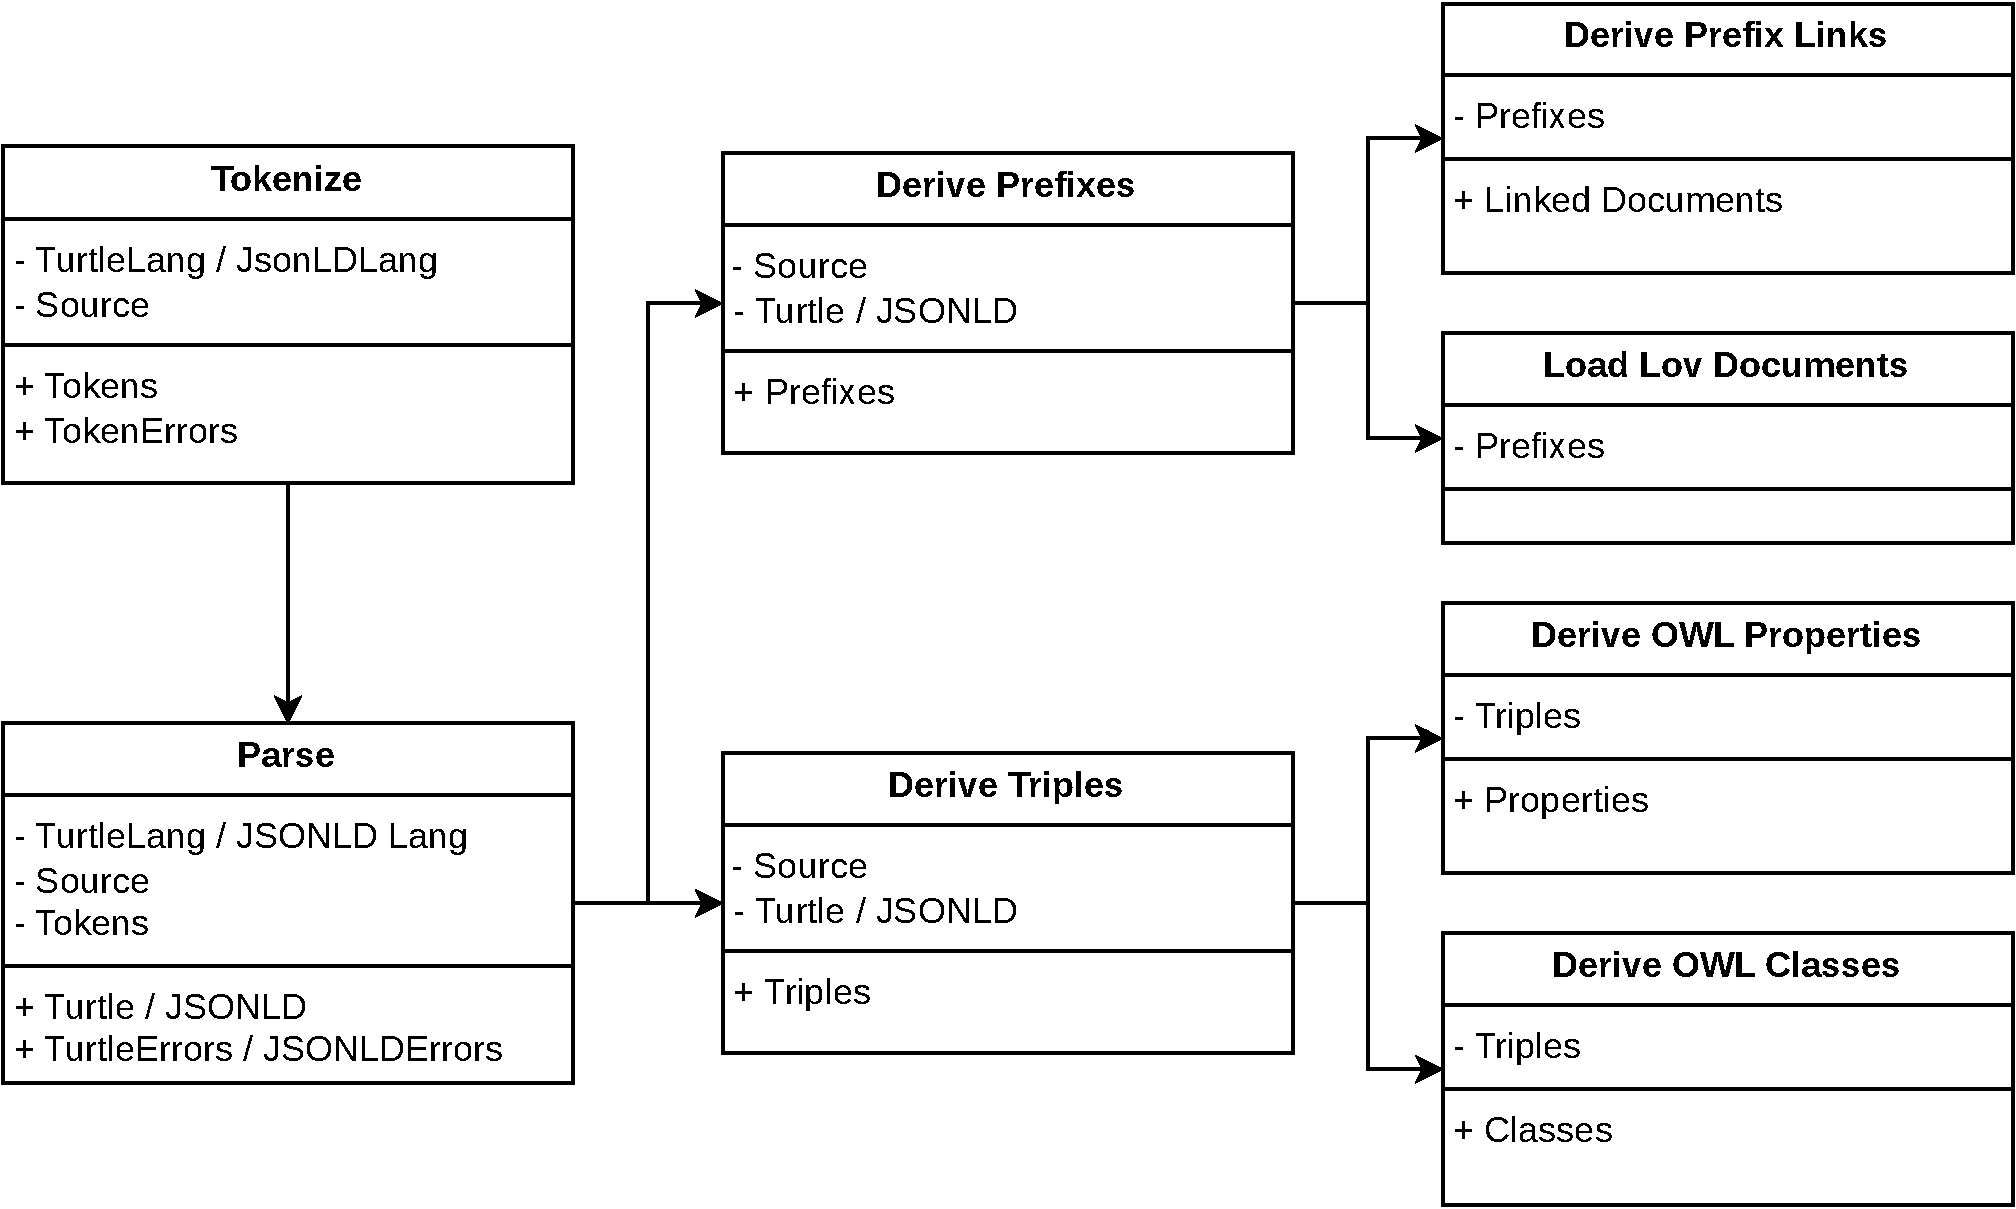
\includegraphics[width=1.2\textwidth]{./images/ParseSchedule.pdf}
 }
  \caption{Visual representation of the Parse schedule including tokenization, parsing, deriving prefixes, deriving triples, linking documents, fetching LOV documents, deriving properties and deriving classes. }\label{fig:Parse}
\end{figure}

We chose to let all semantic languages use the same \texttt{token} type, this allows for implementing token based systems only once.
Note that each semantic language does it's own tokenization, not allowing for SPARQL tokens inside Turtle documents.
In Figure \ref{fig:Parse}, \textit{tokenize} is the first sytem in the parsing schedule, this system is implemented for all supported semantic languages. \textit{Tokenize} also report on tokenization errors.

The next system is \textit{parsing}, also implemented for each semantic language, transforming the tokens into actual objects, and reporting on syntactic errors. 
When the objects are parsed, systems are issued that derive prefixes and triples. 
Prefixes contain information about how to expand and shorten iri's for the current document.
Deriving triples does not only derive actual triples, but in the case for SPARQL also bindings, which can be thought of as \textit{triples}.

After deriving prefixes, other systems will create a \texttt{LinkedDocuments} component, listing all documents that are linked some way to this document.
Prefixes are one way, but the object value of the triple \texttt{<> owl:imports <otherLocation>.}, also linkes that other document with the current document.
Prefixes are also used to load the correct LOV defined ontologies, setting up documents containing property and class definitions.

When the triples are derived, a system will derive properties and classes.
In most documents this will result in no properties or classes, but a document linked from LOV will contain many.
The power of the entity component system is that all documents are handled exactly the same.
This allows to cover a use case where a domain expert is writing the ontology and creating SPARQL queries to see how the ontology \textit{feels}, just by importing a local ontology file.

\paragraph{Some words on parsing}

With the language server protocol the server can specify wether or not it requires only the (minimal) changes or entire document every time.
Earlier versions of the semantic lsp required the entire document every time, because documents arae relatively small and reprasing the entire document brings an acceptable performance.
However, we noticed that this hampered the implementation, in turtle specifically there are patterns that cannot be parsed correctly and brings incorrect and frustrating feedback to the user, and partial parsing helps in this regard.
An example is shown in \ref{lst:GroupedListing}.
  The user at \ref{code1} types named node \texttt{<b>}, the language server should not be confused: triple \texttt{<c> <d> <e>} has nothing to do with named node \texttt{<b>}. The language server should suggest objects that fulfill the domain of predicate \texttt{<b>}. 
  The user at \ref{code2} types named node \texttt{<c>}, the language server should not be confused: the are two triples \texttt{<a> <b> <c>} and \texttt{<a> <d> <e>}, however tokenwise the documents are the same. Resulting in the language server suggesting a semi colon.
  
  The user at \ref{code3} just wrote a subject, invocing the subject completion defined in the next section. The language server might incorrect suggest to add a comma after \texttt{<c>} to build a syntactically correct document.
  The user at \ref{code4} is typing a predicate for the subject \texttt{<a>}, the language server might incorrectly parse the document as seen at \ref{code3}, where \texttt{<b>} is subject thus not invocing the property completion as explained in the next section.

  Adding partial parsing eliminates these issues as the language server understand which tokens are new and leaving the original interpretation of the surrounding tokens in touch.


\begin{figure}[tb]
    \centering
    % code1
    \begin{subfigure}{0.21\textwidth}
      \lstinputlisting{./code/option1.ttl}
      \caption{User types \texttt{<b>}}
      \label{code1}
    \end{subfigure}
    \hfill
    % code 2
    \begin{subfigure}{0.21\textwidth}
      \lstinputlisting{./code/option2.ttl}
      \caption{User types \texttt{<c>}}
      \label{code2}
    \end{subfigure}
    \hfill
    % code 3
    \begin{subfigure}{0.21\textwidth}
      \lstinputlisting{./code/option3.ttl}
      \caption{User types \texttt{<a>}}
      \label{code3}
    \end{subfigure}
    \hfill
    % code 4
    \begin{subfigure}{0.21\textwidth}
      \lstinputlisting{./code/option4.ttl}
      \caption{User types \texttt{<b>}}
      \label{code4}
    \end{subfigure}
    \caption{Different code samples showing that it is the indentation/intent of the user that dictates how tokens should be parsed. (a) and (b) show five terms that result in different triples. (c) and (d) show four terms, triples with subject \texttt{<a>} and \texttt{<b>} and both triples with subject \texttt{<a>} resulting in different semantics.    }\label{lst:GroupedListing}
\end{figure}



\subsubsection*{Completion}

Completion is one of the most important features that actively interacts with the user.
In the Langauge Server Protocol, the langauge server is issed a completion event that contains the current location of the user.
The server should then answer with a list of completions, including the textual operations, a title and potentially some documentation.
It's the responsibility of the editor to sort and filter the completions and show the user the most relevant information.
How editors do this is not specified, which makes it difficult to create comprehensive testing suite.

\begin{figure}[!ht]
 \centering
 \makebox[\textwidth]{%
    \includegraphics[width=1.2\textwidth]{./images/Completion.pdf}
 }
  \caption{Visual representation of our example pipeline, 
      loading sensor data from The Things Network into a triple store}\label{fig:Completion}
\end{figure}

Figure \ref{fig:Completion} shows a schematic overview of the different systems in the completion schedule and their interactions.
First the server will create a \texttt{CompletionRequest} object, currently containing no completions.
Systems add their relevant completions to the request which is then returned to the user.

The location the user at the moment of the request is not enough information to derive comprehensive completions, 
the first systems will extract more information that is then used by the systems that create the actual completions.

\texttt{GetCurrentToken} expands the current location to the current token, then \texttt{GetCurrentTriple} tries to find the triple that this token corresponds to also indicating whether the user is typing a subject, predicate or object.
If \texttt{GetCurrentToken} fails, the entity lacks a TokenComponent and results in \texttt{GetCurrentTriple} not being issued.

The language server has enough information with only the current token to complete based on defined subjects with the \texttt{SubjectCompletion} system.
The server also completed on already defined prefixes (with \texttt{CompletePrefix}), this system is language agnostic as the Prefixes component is already defined.
To import new prefixes from LOV, each language has to implement a \texttt{CompleteLOVPrefix}, because how to add the import statement is language specific.


\subsubsection*{Diagnostics}




\subsubsection*{SemanticHighlighting}

